\tikzset{-, every picture/.style={line width=0.75pt}} %set default line width to 0.75pt        
\begin{figure}[H]
    \centering
    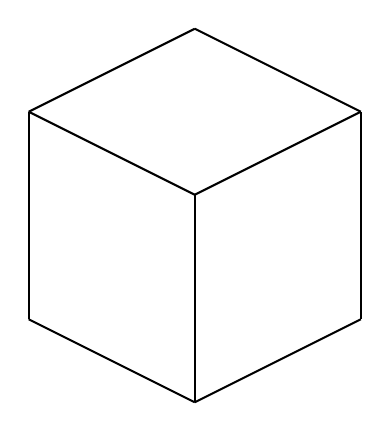
\begin{tikzpicture}[x=0.75pt,y=0.75pt,yscale=-1,xscale=1]
        %uncomment if require: \path (0,300); %set diagram left start at 0, and has height of 300

        %Straight Lines [id:da052099186519106055] 
        \draw    (234,86) -- (234,186) ;
        %Straight Lines [id:da6296181006552015] 
        \draw    (234,86) -- (314,126) ;
        %Straight Lines [id:da34479128766647027] 
        \draw    (314,126) -- (394,86) ;
        %Straight Lines [id:da7728351637240529] 
        \draw    (314,46) -- (234,86) ;
        %Straight Lines [id:da3095482376565484] 
        \draw    (314,46) -- (394,86) ;
        %Straight Lines [id:da019510812171401604] 
        \draw    (234,186) -- (314,226) ;
        %Straight Lines [id:da7918604023131788] 
        \draw    (394,186) -- (314,226) ;
        %Straight Lines [id:da43921670234898924] 
        \draw    (394,86) -- (394,186) ;
        %Straight Lines [id:da07253833503340212] 
        \draw    (314,126) -- (314,226) ;

    \end{tikzpicture}
    \caption{Trimetric projection}
    \label{fig:trimetric}
\end{figure}
% make trimetric